\documentclass{resonance}
\usepackage[hidelinks]{hyperref}
\usepackage{xcolor}
\usepackage[cache=false]{minted}
\usepackage{float}
\usemintedstyle{xcode}
\raggedbottom
\setlength{\fboxsep}{0pt}

\begin{document}
	
	\title{Mathematical Simulation using Monte Carlo Method}
	\secondTitle{Approximation of Pi using Flutter}
	\author{Akshansh Bhanjana - Aryan Gupta}
	
	\maketitle
	\authorIntro{\includegraphics[width=2cm]{akshansh}\\
		Akshansh Bhanjana is a sophomore at Cluster Innovation Centre,
		University of Delhi, currently majoring in Information Technology and Mathematical Innovations.\\
		\authorIntro{\includegraphics[width=2cm]{aryan}\\
			Aryan Gupta is a student at Cluster Innovation Centre,
			University of Delhi, pursuing majors in Information Technology \& Mathematical Innovations.}}
	
	\begin{abstract}
		Algorithms involving Monte Carlo Methods are comparatively scalable. They see a lot of usage in physical systems. This paper involves a Monte Carlo simulation to estimate the value of Pi, written in an open source language, Dart.
	\end{abstract}
	
	\monthyear{June 2020}
	\artNature{GENERAL ARTICLE}
	
	
	\section{Introduction}
	In real life, we encounter various situations where an analytical solution cannot be calculated directly. This calculation may be difficult due to various reasons such as having many random variables, disturbances (noise) in the observations, etc.
	
	Monte Carlo methods are a class of computational algorithms which rely on repeated random sampling to obtain numerical results. The underlying concept is to use randomness to solve problems that might be deterministic in nature.
	
	The core meaning of a Monte Carlo simulation is that we can get an unbiased representative group of samples from a large ocean of possibilities if we allow the simulation to evolve randomly.
	
	The Monte Carlo Method came into existence around the 1940s by scientists involved in The Manhattan Project (which led to the development of the atomic bomb). Named after Monaco, a city infamous for its casinos and games of 'chances', its purpose was to use random input samples to understand a complex system. 
	
	Nowadays, the Monte Carlo method provides usage in a wide range of risk analysis problems in almost every industry. These use-cases find prominence in professional fields such as finance, engineering, R\&D and more.
	
	\section{The Concept}
	In Mathematics, we usually find analytical solutions to problems in order to determine the exact worth i.e quantity, price etc. However, in real life, we rarely find an analytical solution to a problem as real life involves a sense of uncertainty, and randomness.
	
	For instance, forecasting, although fairly uncertain, is typically communicated as single precise average numbers. These exact averages escalate into a number of systematic errors, which are referred to as the \emph{Flaw of Averages}.
	
	Consider a classic problem: a bold Statistician trying to cross a river (Figure 1).
	
	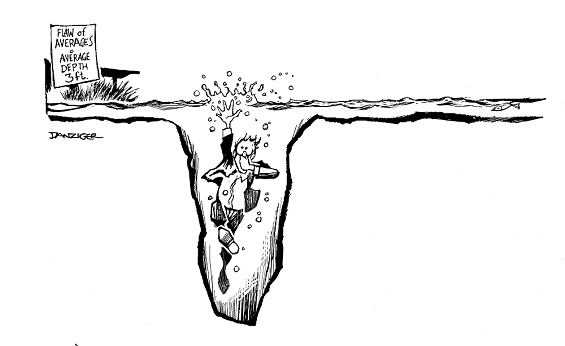
\includegraphics[width=10cm]{the-flaw-of-averages}
	
	\scriptsize{\textbf{Figure 1}. The Flaw of Averages (Source: Sam L. Savage, Hoboken, NJ: John Wiley \& Sons, 2009)}
	
	\normalsize
	The Statistician deems the river safe to cross based on the sign which declares the average depth of the river to be 3 feet. However, in reality, the river is only 6 inch deep around the banks, but 8 feet deep at the centre. The foolhardy statistician drowns clinging on to the f(law) of averages.
	
	The \emph{Flaw of Averages}, formulated by Sam Savage states that 'A plan based on average assumptions is wrong, on average.'
	
	Thus, taking a numerical value as a substitute for an uncertainty does not constitute for random variations. This is where the Monte Carlo Method steps in, providing accuracy over ‘single-point’ estimate analysis.
	
	Monte Carlo Method achieves this by applying the Law of Large Numbers; which quite rightly states, that 'An average tends to come closer to its expected value the more samples we have.'
	
	The percentage error of Monte Carlo Method is inversely proportional to $\sqrt{n}$, where n is the number of random samples. As the number of samples increase, the percentage error decreases.
	
	Therefore, two important components of Monte Carlo are the random samples, and the large number of random samples.
	
	Monte Carlo Method can be best understood through visualization. Using the Monte Carlo Method, it becomes possible to find probability distributions involving random variables, using simulations, known as Monte Carlo simulations. These algorithmic simulations depend on repeated random samplings to get approximate analytical results.
	
	Mathematically, The Monte Carlo Method has 3 use cases:
	\begin{itemize}
		\item \textbf{estimating} probability distribution of a function
		\item \textbf{approximating} mean, variance, or other such quantities
		\item \textbf{optimizing} functions, i.e. maximizing / minimizing functions
	\end{itemize}
	
	\section{Mathematical Foundation}
	The Law of Large Numbers states that with the increase in the number of random trials, the estimated quantity becomes more accurate.\textsuperscript{[2]}
	
	The Monte Carlo Method approximates a property of a huge distribution, by averaging that property for N of these chosen at random i.e. through drawing samples. Drawing a sample may involve the calculation of the probability of a random event or a computational simulation i.e. Monte Carlo Simulation.\textsuperscript{[3]}
	
	Monte Carlo Methods can be expressed in \textit{mathematical terms} as follows:
	
	Consider a multi-dimensional random variable, \textbf{X}, with its Probability Density Function (PDF) as \textbf{f\textsubscript{X}(x)}. Then, the expected value of the function \textbf{g(X)}\textsuperscript{[4]} is:
	
	$$E(g(X)) = \sum_{x\varepsilon X} g(x)f\textsubscript{X}(x);\ if\ X\ is\ discrete$$
	$$E(g(X)) = \int_{x\varepsilon X} g(x)f\textsubscript{X}(x);\ if\ X\ is\ continuous$$
	
	Taking an N-sample of X’s, and computing the mean of \textbf{g(x)} over the sample, the Monte Carlo Approximation equals:
	
	$$ \overline{g}\textsubscript{n}(x) = \frac{1}{n} \sum_{i=1}^{n}g(x\textsubscript{i}) $$
	
	\section{Monte Carlo Error Analysis}
	The Monte Carlo method clearly yields approximate results. The accuracy deppends on the number of values $N$ that we use for the average. A possible measure of the error is the \emph{variance} $\sigma^2$ defined by:
	
	$$ \sigma^2 = \langle f^2 \rangle - \langle f \rangle^2 $$
	
	where
	
	$$ \langle f \rangle = \frac{1}{N} \sum_{i=1}^{n}f(x\textsubscript{i}) $$
	
	and
	
	$$ \langle f^2 \rangle = \frac{1}{N} \sum_{i=1}^{n}f(x\textsubscript{i})^2 $$
	
	The \emph{standard deviation} is $\sigma$. However, the error decreases with the number of points $N$, but the quantity $\sigma$ defines does not. Hence, this cannot be a good measure of the error.
	
	Imagine that we perform several measurements of the integral, each of them yielding a result $I\textsubscript{n}$. These values have been obtained with different sequences of $N$ random numbers. According to the central limit theorem, these values would be normally dstributed around a mean $\langle I \rangle$. Suppose that we have a set of $M$ such measurements ${I\textsubscript{n}}$. A convenient measure of the differences of these measurements is the \emph{standard deviation of the means} $\sigma\textsubscript{M}$:
	
	$$ \sigma^2\textsubscript{M} = \langle I^2 \rangle - \langle I \rangle^2 $$
	
	where
	
	$$ \langle I \rangle = \frac{1}{M} \sum_{n=1}^{M}I\textsubscript{n} $$
	
	and
	
	$$ \langle I^2 \rangle = \frac{1}{M} \sum_{n=1}^{M}I^2\textsubscript{n} $$
	
	Although $\sigma_M$ gives us an estimate of the actual error, making additional measurements is not practical. Instead, it can be proven that:
	
	$$ \sigma\textsubscript{M} \approx \sigma/\sqrt{N} $$
	
	This relation becomes exact in the limit of a very large number of measurements.\textsuperscript{[5]}
	
	\section{Algorithmic/Computer Implementation (Estimating Pi)}
	
	The plan is to simulate random \textbf{(x, y)} points on a 2-D plane with the domain as a square of side \textbf{2R} units. Consider a circle inside the same domain with the same diameter and inscribed into the square. Basically,
	
	$$\frac{area\ of\ the\ circle}{area\ of\ the\ square}\ =\ \frac{number\ of\ points\ inside\ the\ circle}{total\ number\ of\ points\ generated}\ =\ \frac{\Pi r\textsuperscript{2}}{4r2}\ =\ \frac{\Pi}{4}\ =\ k$$
	
	that is,
	
	\authorIntro{
		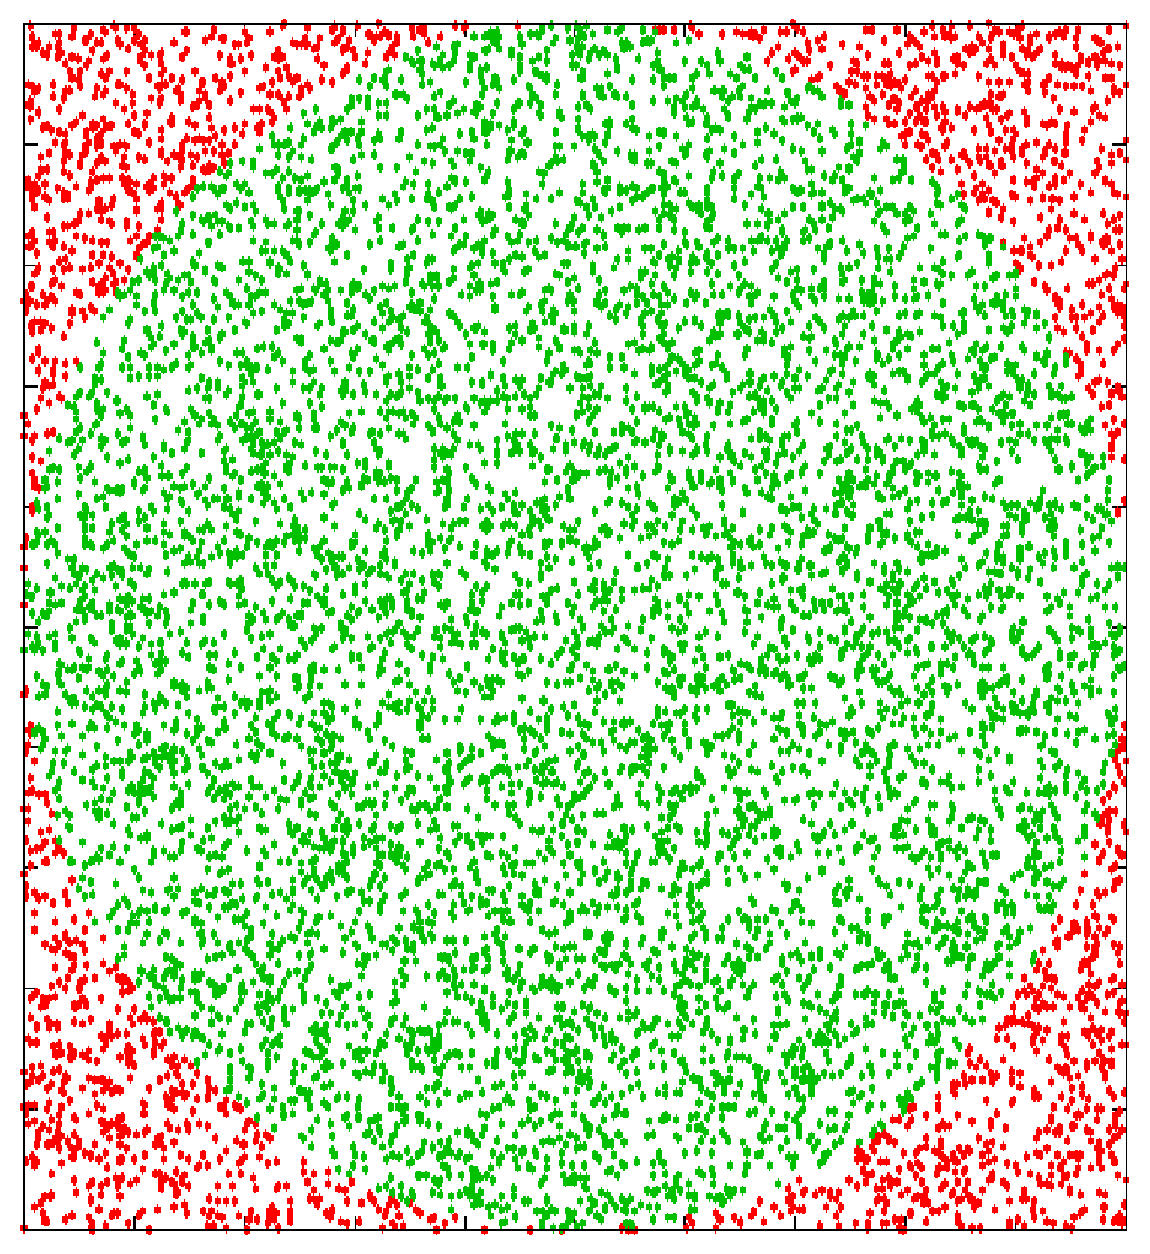
\includegraphics[width=3.5cm, height=3.5cm]{pi}\\
		\scriptsize{Figure 2. \normalfont Distribution of randomly plotted points between -R and R\\
			(Source: \\
			\textcolor{blue}{\url{www.physics.smu.edu}})}
		}
	
	$$\Pi\ =\ 4\ *\ k$$
	
	The points are generated in the \textbf{Dart} language using the \textit{dart:math} library, i.e.
	
	$$x\ =\ rand(-R,\ R)$$
	$$y\ =\ rand(-R,\ R)$$
	$$where\ \textbf{rand(a,\ b)}\ generates\ random\ points\ between\ a\ and\ b$$
	
	This is assuming that the centres of both, the square and the circle, lie at the \textbf{origin}.
	
	Now that random points are generated, we start plotting them. If the generated point lies within the circle, we mark it with \textit{green}, else with \textit{red}. The value given by \textbf{4 * k} then evaluates to:
	
	$$\Pi\ =\ 4\ *\ k\ =\ 4\ *\ \frac{number\ of\ green\ dots}{total\ number\ of\ dots\ (green\ +\ red)}$$
	
	The best thing is that we don’t need to consider graphics for simulation. We only need to output random \textbf{(x, y)} pairs and then do the following:
	
	\begin{itemize}
		\item if the point lies inside the circle - increment number of points inside the circle
		\item increment the total number of points irrespective of where the point lies
		\item calculate the above result, i.e. \textbf{4 * k}
	\end{itemize}
	
	To have a clearer view of the above, we have prepared a simulation. Given below are 3 screenshots of the simulation, at 3 different times. The time and the number of plotted points increase from left to right:
	
	\begin{figure}[h!]
		\hskip 0.7cm
		\vspace{20pt}
		\fbox{\includegraphics[width=3cm]{pi_ss_1}}
		\fbox{\includegraphics[width=3cm]{pi_ss_2}}
		\fbox{\includegraphics[width=3cm]{pi_ss_3}}
		
		\vspace{-10pt}
		\hspace{30pt}\scriptsize{\textbf{Figure 3}. \normalfont Simulating the Approximation of Pi, density increasing with time}\\
	\end{figure}

	\rightHighlight{For reference, the video is hosted at \textcolor{blue}{\url{https://youtu.be/xaFbJSVc4cc}}}
	
	In the above, it is clearly evident that as the number of points increases, the approximate value of Pi approaches the real value. This is in complete agreement with the hypotheses above, and hence, proves that Monte Carlo simulations are good approximations when one can’t calculate the exact value.
		
	\section{Result}

	\rightHighlight{For reference, a colab notebook containing the error analysis code is available at \textcolor{blue}{\url{https://bit.ly/pi-approx-errors}}}

	The results of the above simulation have been scatter-plotted, with the X-axis as $1/\sqrt{N}$ and Y-axis as the percentage error. It can be observed that the percentage error reduces in proportion to $1/\sqrt{N}$.
	
	\begin{figure}[H]
		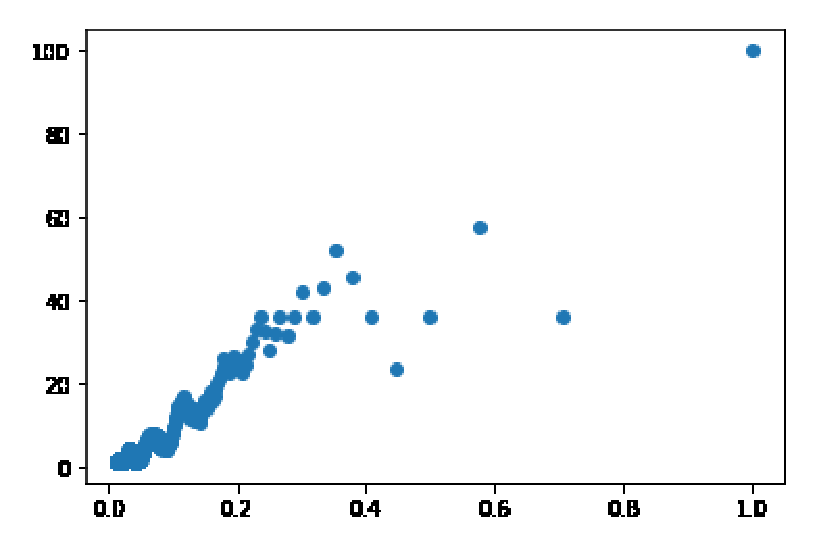
\includegraphics[width=10cm]{error-plot}
	\end{figure}
	\vspace{-10pt}\hspace{10pt}\scriptsize{\textbf{Figure 4}. The relation between percentage error and $1/\sqrt{N}$, where $N = number\ of\ darts$}

	\normalsize
	\section{Conclusion}
	In this paper, a Monte Carlo simulation has been used to estimate the value of $\pi$.
	
	The Monte Carlo Method has been shown to be valid and effective, through testing at various parameters.
	
	Moreover, the simulation has proved to deliver satisfactory and expected results, whilst clearly demonstrating the feasibility of the Monte Carlo Method. These methods hold great promise in the future of AI, and have already forayed into the world of deep-learning.
	
	\section{Resources}
	The entire code for the above simulation (along with the Flutter project) can be found at:\\ \textcolor{blue}{\url{https://github.com/akshansh2000/pi_approximation}}.
	
	To see the project in action online, one can refer to the dartpad (make sure to turn off \emph{Null Safety} from the bottom bar):\\
	\textcolor{blue}{\url{https://dartpad.dev/8eea3f7534658c9a54b8ebd7c37487db}}
	
	\pagebreak
	\begin{thebibliography}{99}
		
		\vspace{5pt}
		\bibitem{latexcompanion}
		“A Gentle Introduction to Monte Carlo Sampling for Probability”\\ \textcolor{blue}{\url{https://machinelearningmastery.com/monte-carlo-sampling-for-probability}}\\
		{[Accessed: 7-April-2020]}\\
		
		\bibitem{latexcompanion}
		"Monte Carlo Simulations”\\ \textcolor{blue}{\url{https://www.palisade.com/risk/monte_carlo_simulation.asp/}}\\
		{[Accessed: 10-April-2020]}\\
		
		\bibitem{latexcompanion}
		"Monte Carlo Methods and Importance Sampling”\\ \textcolor{blue}{\url{http://ib.berkeley.edu/labs/slatkin/eriq/classes/guest\_lect/mc\_lecture\_notes.pdf}}\\
		{[Accessed: 2-May-2020]}\\
		
		\bibitem{latexcompanion}
		"Mathematical Foundations of Monte Carlo Methods”\\ \textcolor{blue}{\url{https://www.scratchapixel.com/lessons/mathematics-physics-for-computer-graphics/monte-carlo-methods-mathematical-foundations/pdf-and-cdf}}\\
		{[Accessed: 12-April-2020]}\\
		
		\bibitem{latexcompanion}
		"Monte Carlo error analysis”\\ \textcolor{blue}{\url{https://web.northeastern.edu/afeiguin/phys5870/phys5870/node71.html}}\\
		{[Accessed: 16-January-2021]}\\
		
	\end{thebibliography}
	
\end{document}
